
\begin{definition}
    Let $B^d$ be the unit ball in $d$ dimensions, $S^d$ be the sphere defining the surface of $B^d$.
    A \textbf{sphere preserving map} from $S^d$ to $S^d$ is a continuous function that sends every low-dimension sphere contained in $S^d$ to a sphere in $S^d$, such that every sphere in $S^d$ has a pre-image under the map that is also a sphere. 
\end{definition}
We consider the stereographic projection between the plane and the sphere. For any point $\alpha \in S^d$, we define $\Pi_\alpha$ to be the stereographic projection from the plane perpendicular to $S^d$ at $\alpha$, and let $\Pi_\alpha^{-1}$ be its inverse. We could show that these two functions are sphere-preserving maps \cite{HCV52}.

We then could obtain sphere-preserving maps in the sphere by applying a projection onto a plane, then dilation of the plane, and then mapping back by stereographic projection. For $\alpha \in S^d$ and $a \geq 0$, we define $D^a_\alpha$ to be the map that dilates the hyperplane perpendicular to $S^d$ at $\alpha$ by a factor $a$. 

As the composition of sphere-preserving maps is also a sphere-preserving map, we now define the sphere-preserving map we will user. For any $\alpha$ such that $\|\alpha\|<1$, define $f_\alpha(z)$ by 
\begin{align*}
    f_\alpha(z) = \Pi_{\alpha/\|\alpha\|}(D_{\alpha/\|\alpha\|}^{1-\|\alpha\|}(\Pi_{\alpha/\|\alpha\|}^{-1})(z))
\end{align*}



% \begin{figure}
% 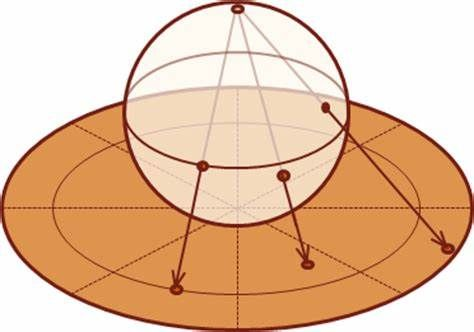
\includegraphics[width=0.4\textwidth]{figures/stereographic.jpg}
% \end{figure}

% A sphere preserving map could be constructed using $\Pi \circ D \circ \Pi^{-1}$, where D is a dilation function


\begin{definition}
    An arrangement of caps ${C_1, ..., C_n}$ in $S^d$ is well-behaved if there is no point that belongs to at least half of the caps.     
\end{definition}
\begin{remark}
    All of the arrangements of caps obtained from graphs contained in the other sections of this report are well-behaved. Otherwise, the induced graphs would have cliques on half o their vertices and no small separators.
\end{remark}

\begin{lemma}
    Let $\phi: B^d \rightarrow B^d$ be a continous function such that, for all $\alpha \in S^d$, $\phi(\alpha)$ lies on the line cnnecting $\alpha$ with $\vzero$ and is closer to $\alpha $ than to $-\alpha$, then there  exists an $\alpha \in B^d$ such that $\phi(\alpha)=\vzero$.  
\end{lemma}\label{le:alpha_exists}
\begin{proof}
We could prove this via contradiction. Assume that there is no point $\alpha \in B^d$ that satisfies $\phi(\alpha)=\vzero$. Consider the map $b(\phi(\alpha))=\phi(\alpha)/\|\phi(\alpha)\|$ with the domain being $B^d - \{\vzero\}$. Since $b$ is a continuous map, $b \circ \phi$ is also a continuous map from $B^d$ onto $S^d$ which is the identity on $S^d$. Therefore, $g(z) = -b(\phi(z))$ is a map from $B^d$ onto $S^d$ that has no fixed point, which contradicts the Brouwer's Fixed Point Theorem, saying that every continuous map from $B^d$ to $B^d$ has a fixed point. 
\end{proof}

With this Lemma, now we could show that we can always find an $\alpha$ and its corresponding map on caps so that the centroid of the centers of their images is at the origin. 

\begin{theorem}
    For any well-behaved arrangement of caps ${C_1, ..., C_n}$ in $S^d$, there is a sphere-preserving map $f_\alpha$ such that the centroid of the centers of $f_\alpha(C_1),f_\alpha(C_2),...,f_\alpha(C_n)$
\end{theorem}\label{th:sum_is_origin}

\begin{proof}
We want to show that there is an $\alpha$ that $\|\alpha\| < 1$ and $\sum_{i=1}^{n}p(f_\alpha(C_i))=\vzero$.
Consider the map from $\alpha$ to the centroid of $\{p(f_\alpha(C_1)), p(f_\alpha(C_2)), ..., p(f_\alpha(C_n))\}$, we want to show that $\vzero$ has a pre-image under this map.

However, the map is not continuous, as when $\|\alpha\| =1$, $-\alpha$ crosses the boundary of $C_i$, and $p(f_\alpha(C_i))$ jumps from one side of the sphere to the other. 

In order to fix this, we construct a modified map that is continous, As the set of caps is well-behaved, we can choose an $\epsilon > 0$ such that for all $\alpha$ that $\|\alpha\| \geq 1-epsilon$, most of the caps $\{(f_\alpha(C_1), f_\alpha(C_2), ..., f_\alpha(C_n)\}$ are entirely contained within the ball of radius $1/2n$ around $\alpha /\|\alpha\|$. As a result, $f_\alpha$ does not map the centroid of the centers of the caps to the origin. For $\alpha \in B^d$, we could define the map as 
\begin{align*}
    \phi(\alpha) = \frac{\sum_{i=1}^{n}w(C_i,\alpha)p(f_\alpha(C_i))}{n}
\end{align*}
where the weight function is 
\begin{align*}
    w(C, \alpha) =  \begin{cases} 
      (2-d(\alpha,C))/\epsilon & d(\alpha,C)\geq 2-\epsilon \\
       1 & otherwise 
   \end{cases}
\end{align*}
The $d(\alpha,C)$ here represents the greatest distance from $\alpha$ to a point in the cap $C$. Since $w$ here is a continuous function that goes to zero as $-\alpha$ approaches the boundary of a cap, $\phi(\alpha)$ is also a continuous function.  

Since we know that $\{C_1, ..., C_n\}$ is well-behaved, it is easy to verify that, for $\alpha \in S^d$, $\phi(\alpha)$ lies on the line connecting $\vzero$ to $\alpha$ and is closer to $\alpha$ compared with $-\alpha$. By Lemma~\ref{le:alpha_exists}, we can find a $\alpha$ such that $\phi(\alpha)=\vzero$.
\end{proof}